\documentclass[]{article}
\usepackage[left=1in,top=1in,right=1in,bottom=1in]{geometry}


%%%% more monte %%%%
% thispagestyle{empty}
% https://stackoverflow.com/questions/2166557/how-to-hide-the-page-number-in-latex-on-first-page-of-a-chapter
\usepackage{color}
% \usepackage[table]{xcolor} % are they using color?

% \definecolor{WSU.crimson}{HTML}{981e32}
% \definecolor{WSU.gray}{HTML}{5e6a71}

% \definecolor{shadecolor}{RGB}{248,248,248}
\definecolor{WSU.crimson}{RGB}{152,30,50} % use http://colors.mshaffer.com to convert from 981e32
\definecolor{WSU.gray}{RGB}{94,106,113}

%%%%%%%%%%%%%%%%%%%%%%%%%%%%

\newcommand*{\authorfont}{\fontfamily{phv}\selectfont}
\usepackage{lmodern}


  \usepackage[T1]{fontenc}
  \usepackage[utf8]{inputenc}




\usepackage{abstract}
\renewcommand{\abstractname}{}    % clear the title
\renewcommand{\absnamepos}{empty} % originally center

\renewenvironment{abstract}
 {{%
    \setlength{\leftmargin}{0mm}
    \setlength{\rightmargin}{\leftmargin}%
  }%
  \relax}
 {\endlist}

\makeatletter
\def\@maketitle{%
  \pagestyle{empty}
  \newpage
%  \null
%  \vskip 2em%
%  \begin{center}%
  \let \footnote \thanks
    {\fontsize{18}{20}\selectfont\raggedright  \setlength{\parindent}{0pt} \@title \par}%
}
%\fi
\makeatother







\usepackage{graphicx,grffile}
\makeatletter
\def\maxwidth{\ifdim\Gin@nat@width>\linewidth\linewidth\else\Gin@nat@width\fi}
\def\maxheight{\ifdim\Gin@nat@height>\textheight\textheight\else\Gin@nat@height\fi}
\makeatother
% Scale images if necessary, so that they will not overflow the page
% margins by default, and it is still possible to overwrite the defaults
% using explicit options in \includegraphics[width, height, ...]{}
\setkeys{Gin}{width=\maxwidth,height=\maxheight,keepaspectratio}


\title{\textbf{\textcolor{WSU.crimson}{Will vs
Denzel.}} \newline \textbf{\textcolor{WSU.gray}{Who is a better
actor?}}  }
 

%  

% \author{ \Large true \hfill \normalsize \emph{} }
\author{\Large Nahom
Debela\vspace{0.05in} \newline\normalsize\emph{Washington State
University}  }


\date{December 14, 2020}
\setcounter{secnumdepth}{3}

\usepackage{titlesec}
% See the link above: KOMA classes are not compatible with titlesec any more. Sorry.
% https://github.com/jbezos/titlesec/issues/11
\titleformat*{\section}{\bfseries}
\titleformat*{\subsection}{\bfseries\itshape}
\titleformat*{\subsubsection}{\itshape}
\titleformat*{\paragraph}{\itshape}
\titleformat*{\subparagraph}{\itshape}

% https://code.usgs.gov/usgs/norock/irvine_k/ip-092225/


%\titleformat*{\section}{\normalsize\bfseries}
%\titleformat*{\subsection}{\normalsize\itshape}
%\titleformat*{\subsubsection}{\normalsize\itshape}
%\titleformat*{\paragraph}{\normalsize\itshape}
%\titleformat*{\subparagraph}{\normalsize\itshape}

% https://tex.stackexchange.com/questions/233866/one-column-multicol-environment#233904
\usepackage{environ}
\NewEnviron{auxmulticols}[1]{%
  \ifnum#1<2\relax% Fewer than 2 columns
    %\vspace{-\baselineskip}% Possible vertical correction
    \BODY
  \else% More than 1 column
    \begin{multicols}{#1}
      \BODY
    \end{multicols}%
  \fi
}





\usepackage{natbib}
\setcitestyle{aysep={}} %% no year, comma just year
% \usepackage[numbers]{natbib}
\bibliographystyle{./../biblio/ormsv080.bst}



\usepackage[strings]{underscore} % protect underscores in most circumstances




\newtheorem{hypothesis}{Hypothesis}
\usepackage{setspace}


%%%%%%%%%%%%%%%%%%%%%%%%%%%%%%%%%%%%%%%%%%%%%%%%%%%%%
%%% MONTE ADDS %%%

\usepackage{fancyhdr} % fancy header 
\usepackage{lastpage} % last page 

\usepackage{multicol}


\usepackage{etoolbox}
\AtBeginEnvironment{quote}{\singlespacing\small}
% https://tex.stackexchange.com/questions/325695/how-to-style-blockquote


\usepackage{soul}			%% allows strike-through
\usepackage{url}			%% fixes underscores in urls
\usepackage{csquotes}		%% allows \textquote in references
\usepackage{rotating}		%% allows table and box rotation
\usepackage{caption}		%% customize caption information
\usepackage{booktabs}		%% enhance table/tabular environment
\usepackage{tabularx}		%% width attributes updates tabular
\usepackage{enumerate}		%% special item environment
\usepackage{enumitem}		%% special item environment

\usepackage{lineno}		%% allows linenumbers for editing using \linenumbers
\usepackage{hanging}


\usepackage{mathtools}  	%% also loads amsmath
\usepackage{bm}		%% bold-math
\usepackage{scalerel}	%% scale one element (make one beta bigger font)

\newcommand{\gFrac}[2]{ \genfrac{}{}{0pt}{1}{{#1}}{#2} }

\newcommand{\betaSH}[3]{  \gFrac{\text{\tiny #1}}{{\text{\tiny #2}}}\hat{\beta}_{\text{#3}}   }
\newcommand{\betaSB}[3]{              ^{\text{#1}} _{\text{#2}} \bm{\beta} _{\text{#3}}                   }  %% bold
\newcommand{\bigEQ}{  \scaleobj{1.5}{{\ }= } }
\newcommand{\bigP}[1]{  \scaleobj{1.5}{#1 } }





\usepackage{endnotes}  % he already does this ...
\renewcommand{\enotesize}{\normalsize}
% https://tex.stackexchange.com/questions/99984/endnotes-do-not-be-superscript-and-add-a-space
\renewcommand\makeenmark{\textsuperscript{[\theenmark]}} % in brackets %
% https://tex.stackexchange.com/questions/31574/how-to-control-the-indent-in-endnotes
\patchcmd{\enoteformat}{1.8em}{0pt}{}{}

\patchcmd{\theendnotes}
  {\makeatletter}
  {\makeatletter\renewcommand\makeenmark{\textbf{[\theenmark]} }}
  {}{}



% https://tex.stackexchange.com/questions/141906/configuring-footnote-position-and-spacing

\addtolength{\footnotesep}{5mm} % change to 1mm

\renewcommand{\thefootnote}{\textbf{\arabic{footnote}}}
\let\footnote=\endnote
%\renewcommand*{\theendnote}{\alph{endnote}}
%\renewcommand{\theendnote}{\textbf{\arabic{endnote}}}


\renewcommand*{\notesname}{ENDNOTES}

\makeatletter
\def\enoteheading{\section*{\notesname
  \@mkboth{\MakeUppercase{\notesname}}{\MakeUppercase{\notesname}}}%
  \mbox{}\par\vskip-2.3\baselineskip\noindent\rule{.5\textwidth}{0.4pt}\par\vskip\baselineskip}
\makeatother


\renewcommand*{\contentsname}{TABLE OF CONTENTS}

\renewcommand*{\refname}{REFERENCES}


%\usepackage{subfigure}
\usepackage{subcaption}

\captionsetup{labelfont=bf}  % Make Table / Figure bold

%%% you could add elements here ... monte says .... %%%
%\usepackage{mypackageForCapitalH}


%%%%%%%%%%%%%%%%%%%%%%%%%%%%%%%%%%%%%%%%%%%%%%%%%%%%%

% set default figure placement to htbp
\makeatletter
\def\fps@figure{htbp}
\makeatother


% move the hyperref stuff down here, after header-includes, to allow for - \usepackage{hyperref}

\makeatletter
\@ifpackageloaded{hyperref}{}{%
\ifxetex
  \PassOptionsToPackage{hyphens}{url}\usepackage[setpagesize=false, % page size defined by xetex
              unicode=false, % unicode breaks when used with xetex
              xetex]{hyperref}
\else
  \PassOptionsToPackage{hyphens}{url}\usepackage[draft,unicode=true]{hyperref}
\fi
}

\@ifpackageloaded{color}{
    \PassOptionsToPackage{usenames,dvipsnames}{color}
}{%
    \usepackage[usenames,dvipsnames]{color}
}
\makeatother
\hypersetup{breaklinks=true,
            bookmarks=true,
            pdfauthor={Nahom Debela (Washington State University)},
             pdfkeywords = {},  
            pdftitle={Will vs Denzel.: Who is a better actor?},
            colorlinks=true,
            citecolor=blue,
            urlcolor=blue,
            linkcolor=magenta,
            pdfborder={0 0 0}}
\urlstyle{same}  % don't use monospace font for urls

% Add an option for endnotes. -----

%
% add tightlist ----------
\providecommand{\tightlist}{%
\setlength{\itemsep}{0pt}\setlength{\parskip}{0pt}}

% add some other packages ----------

% \usepackage{multicol}
% This should regulate where figures float
% See: https://tex.stackexchange.com/questions/2275/keeping-tables-figures-close-to-where-they-are-mentioned
\usepackage[section]{placeins}



\pagestyle{fancy}   
\lhead{\textcolor{WSU.crimson}{\textbf{ Will vs Denzel. }}}
\chead{}
\rhead{\textcolor{WSU.gray}{\textbf{  Page\ \thepage\ of\ \protect\pageref{LastPage} }}}
\lfoot{}
\cfoot{}
\rfoot{}


\begin{document}
	
% \pagenumbering{arabic}% resets `page` counter to 1 
%    

% \maketitle

{% \usefont{T1}{pnc}{m}{n}
\setlength{\parindent}{0pt}
\thispagestyle{plain}
{\fontsize{18}{20}\selectfont\raggedright 
\maketitle  % title \par  

}

{
   \vskip 13.5pt\relax \normalsize\fontsize{11}{12} 
   
\textbf{\authorfont Nahom Debela} \hskip 15pt \emph{\small Washington
State University}   

}

}








\begin{abstract}

    \hbox{\vrule height .2pt width 39.14pc}

    \vskip 8.5pt % \small 

\noindent \noindent Comparing IMDB data to reveal who the better actor
is between Will Smith and Denzel Washington \vspace{0.12in}


    



    
    \hbox{\vrule height .2pt width 39.14pc}
    \vskip 5pt 
    \hfill \textbf{\textcolor{WSU.gray}{ December 14, 2020 } }
    \vskip 5pt 
    
\end{abstract}


\vskip -8.5pt



 % removetitleabstract

\noindent  

\vspace{5mm}

\noindent In order to find out who the better actor is I had to
determine which features were relevant for comparing these actors. I did
not want to compare the movie profit related to each of the actors
because I believe that a larger profit margin implies more fan appeal,
advertising, or simply popularity. This doesn't answer my research
question of who is the better actor. I couldn't simply choose who had
more movies or who has more experience because that doesn't fit the
definition of `better.' The formal definition of better is ``of a more
excellent or effective type or quality.'' Although these actors are both
talented in their own right, my analysis has led me to the conclusion
that \_\_\_ is a better actor than \_\_\_.

\vspace{3mm}

\begin{figure}[!ht]
    
    \begin{center}
        \scalebox{0.95}{    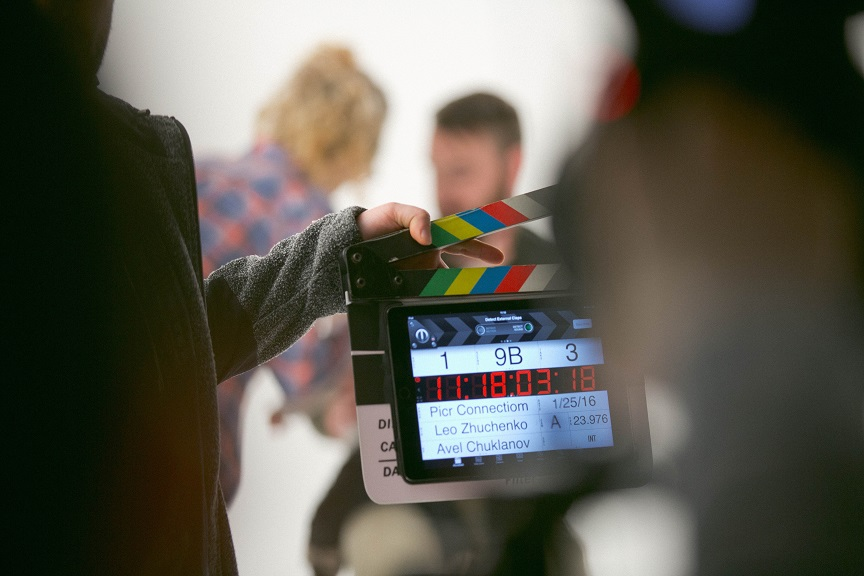
\includegraphics[trim = 0 0 2cm 0,clip,width=0.85\textwidth]{figures/acting.jpg} }
    \end{center}
    \label{fig:handout-1}
    
\end{figure}

\vspace{4mm}

\noindent Both Will Smith and Denzel Washington are currently starring
in films. Will, who is 52 years old began acting in films in 1992. While
Denzel, Who is 60 years old began acting in films in 1981. In this
report I compare these actors by multiple factors both directly relating
to the movies ranking themselves and by the crew members each actor had
available to them. I believe to objectively determine who is a better
actor I must not only compare the actors side by side, but also the
level of help each actor had in the movies. I compared the directors,
co-Stars, and writers of both Will and Denzel's movies to see the true
effectiveness they had in their films.

\newpage
\vspace{4mm}
\subsection{Summary of Sample}
\label{sec:data-sample}

\noindent  \vspace{10mm}

\begin{verbatim}
## Will Smith will has or will act in a total 34 of Movies by around 2021
\end{verbatim}

\begin{verbatim}
## Denzel Washingon has or will act in a total 45 of Movies by around 2021
\end{verbatim}

\begin{verbatim}
## Will Smith has worked alongside: 104 Co Stars
\end{verbatim}

\begin{verbatim}
## Denzel Washington has worked alongside: 138 Co Stars
\end{verbatim}

\begin{verbatim}
## Number of Headlining Co-Stars for Will:  39
\end{verbatim}

\begin{verbatim}
## Number of Headlining Co-Stars for Denzel:  59
\end{verbatim}

\begin{verbatim}
## Number of Popular 50 Co-Stars for Will:  59
\end{verbatim}

\begin{verbatim}
## Number of Popular 50 Co-Stars for Denzel:  83
\end{verbatim}

\begin{verbatim}
## Number of Top 250 Co-Stars for Will:  24
\end{verbatim}

\begin{verbatim}
## Number of Top 250 Co-Stars for Denzel:  34
\end{verbatim}

\begin{verbatim}
## Number of Gem 50 co-Stars for Will:  13
\end{verbatim}

\begin{verbatim}
## Number of Gem 50 co-Stars for Denzel:  22
\end{verbatim}

\begin{verbatim}
## Number of star ranked co Stars for Will:  57
\end{verbatim}

\begin{verbatim}
## Number of star ranked co Stars for Denzel:  71
\end{verbatim}

\begin{verbatim}
## Number of Top Directors for Will:  2
\end{verbatim}

\begin{verbatim}
## Number of Top Directors for Denzel:  9
\end{verbatim}

\begin{verbatim}
## Number of Top Writers for Will:  2
\end{verbatim}

\begin{verbatim}
## Number of Top Writers for Denzel:  5
\end{verbatim}

\begin{verbatim}
## The average rating of movies that have aired featuring Will Smith is: 6.5375
\end{verbatim}

\begin{verbatim}
## The average rating of movies that have aired featuring Denzel Washington is: 6.928571
\end{verbatim}

\newpage
\subsection{Results}
\label{sec:results}
\vspace{10mm}

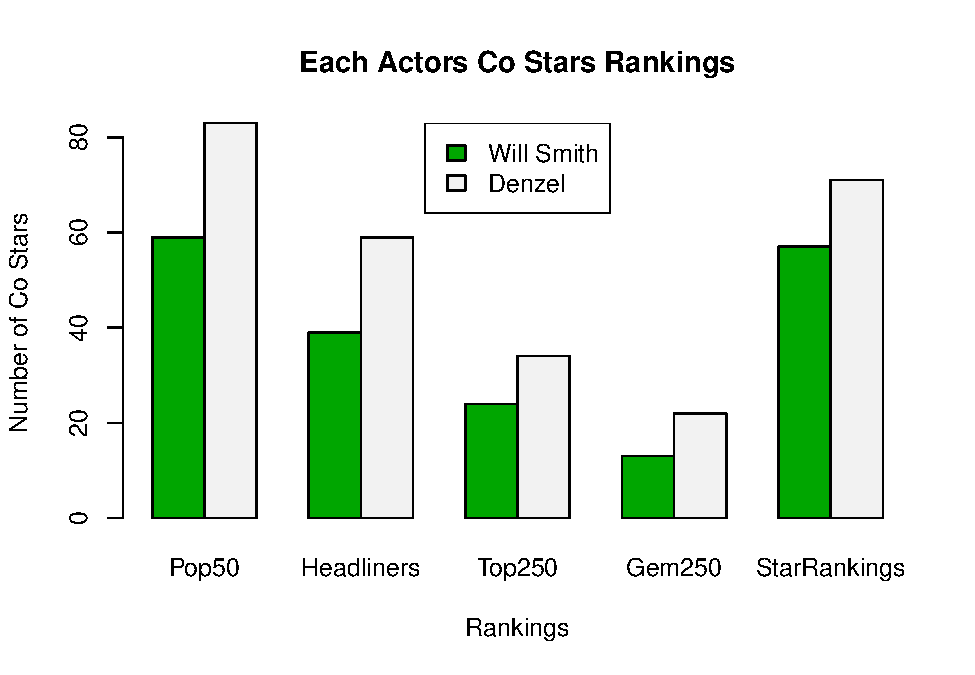
\includegraphics{will-v-denzel_files/figure-latex/codePlot-1.pdf}
\newpage \vspace{10mm}

\subsection{Conclusion}
\label{sec:conclusion}

\noindent In conclusion I pick Will Smith as the better actor over
Denzel Washington. Throughout my analysis I noticed that Denzel
Washington overall had a higher average rating than Will Smith. Both
these actors are very talented, however in order to compare them I must
compare their performances and take into account the talent that was
around them in the process. This is where I noticed a significant
difference between the actors. I decided that because Will Smith had far
less talent around him and only had a slight drop off in average rating:
Will Smith is the better actor. I can suggest that as an actor increases
the talent around them, the ratings of the movies increase. This is
exactly the case between these two actors.

\vspace{7mm}

\noindent Denzel Washington has starred in about 25\% more movies than
Will Smith. Additionally, in every case he has had far more prominent
writers, directors, and co-stars than will smith. Of course this is
expected since he has more movies. However, if these artists had the
same amount of talent around them, the ratio should only be about 4:3.
This is not the case. This was especially noticable in the directors and
writers for these actors. Denzel has had significantly more prominent
directors than Will. Denzel has had 9 directors who have headlined at
least 15 times as a director, compared to Smith's 2. Also Denzel has had
significantly more prominent writers than Will. Denzel has had 5 writers
who have headlined at least 15 times as a writer, compared to Will's 2.
That is about a much larger ratio in favor of Denzel.

\vspace{7mm}

\noindent Overall, It was very difficult to choose between these two
actors. Though undoubtedly, the evidence is there. With less prominent
Co-Stars, Writers and directors Will Smith was able to star in movies
that were on average rated 6.5, compared to Denzels 6.9. That is only a
.4 drop off compared to Denzels average movie rating. This difference is
not all that significant to simply choose Denzel, so, by collecting more
information such as their cast mates rankings I was able to narrow down
the features that determine who the `better' actor is: Will Smith.




%% appendices go here!


\newpage
\theendnotes

%%%%%%%%%%%%%%%%%%%%%%%%%%%%%%%%%%%  biblio %%%%%%%%
\newpage
\begin{auxmulticols}{2}
\singlespacing 
\bibliography{./../biblio/master.bib}

%%%%%%%%%%%%%%%%%%%%%%%%%%%%%%%%%%%  biblio %%%%%%%%
\end{auxmulticols}

\newpage



\end{document}